
\begin{figure}

\begin{minipage}{0.5\textwidth}
\small

\begin{verbatim}
int time;

int [] discovery;
int [] finish;

function visit( Node v ) {
    time = time + 1;
    discovery[id(v)] = time;
    beginStep();
    label(v, discovery[id(v)] );
    select(v);
    endStep();
    for_outgoing( v, e, w ) {
        beginStep();
        if ( ! selected(w) ) {
            select(e);
            visit(w);
        }
        else if ( finish[id(w)] == 0 ) {
            label(e, "B");
        }
        else if ( finish[id(w)] 
                  > discovery[id(v)] ) {
            label(e, "F");
        }
        else {
            label(e, "C");
        }
        endStep();
    }
    time = time + 1;
    finish[id(v)] = time;
    beginStep();
    mark(v);
    label(v, discovery[id(v)]
             + "/" + finish[id(v)]);
    endStep();
}

algorithm {
    time = 0;
    discovery = new int[nodeIds()];
    finish = new int[nodeIds()];
    for_nodes( u ) {
        if ( ! selected(u) ) {
            visit( u );
        }
    }
}
\end{verbatim}
\end{minipage}
\begin{minipage}{0.49\textwidth}
\centering

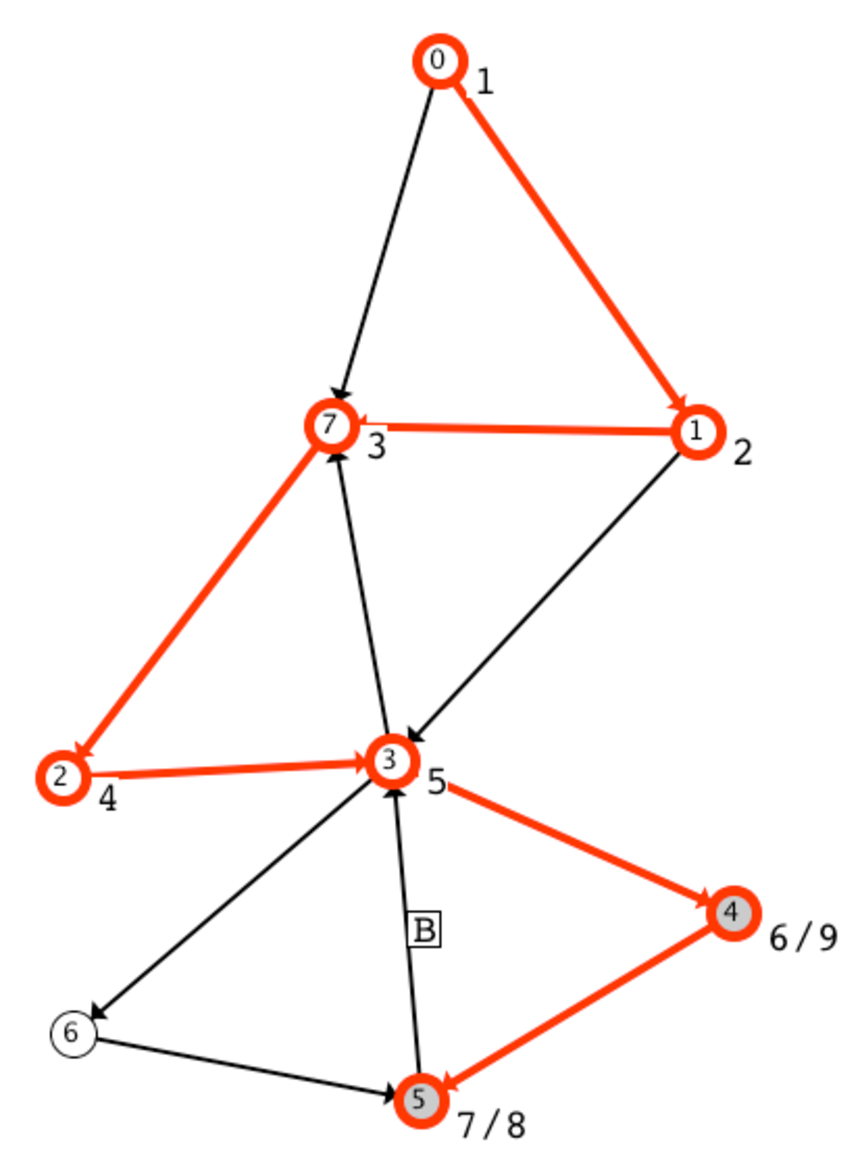
\includegraphics[scale=0.5]{X_dfs_d_1}

After first non-tree edge is labeled. 

\medskip

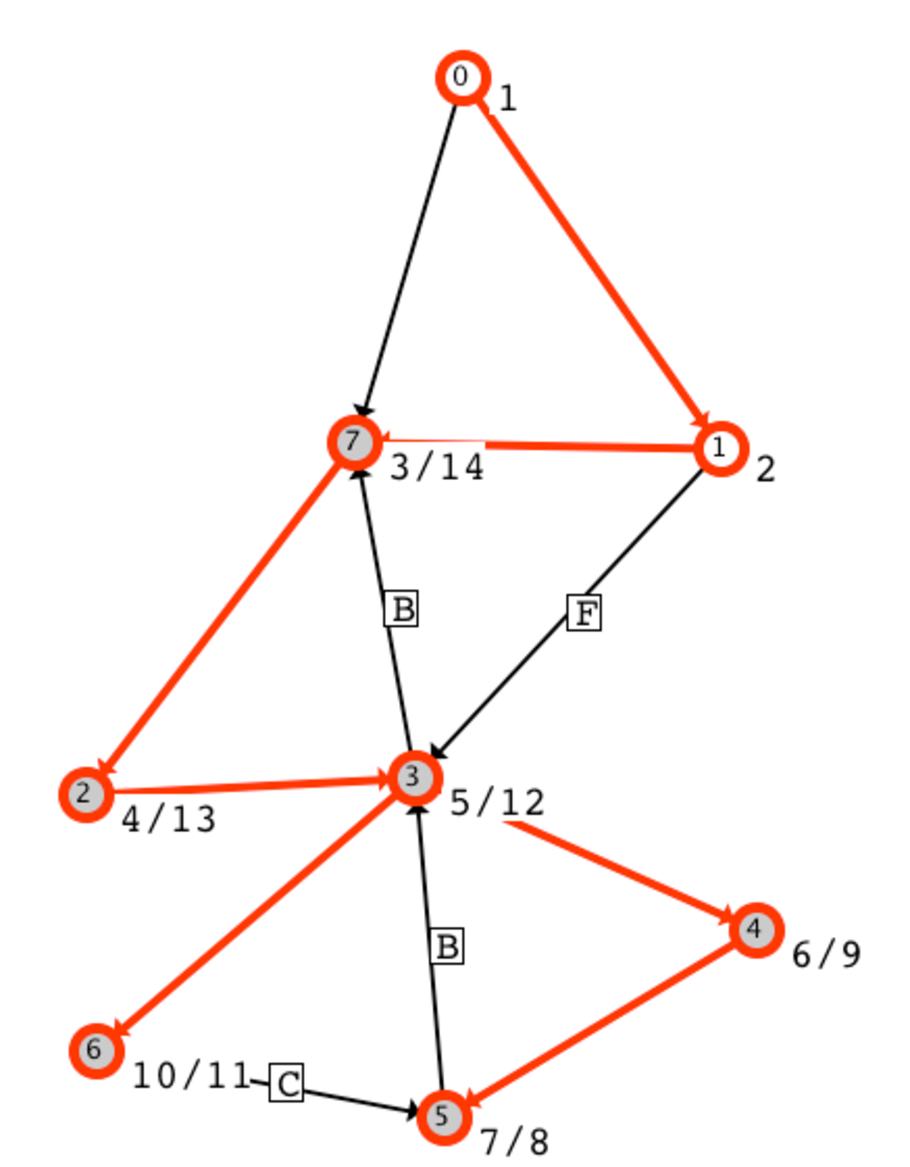
\includegraphics[scale=0.5]{X_dfs_d_2}

After all but one non-tree edges have been labeled.

\end{minipage}
\caption{Implementation of a depth-first search animation
  with an illustration of the graph panel during execution.}
\label{fig:dfs}
\end{figure}
